\documentclass[12pt, a4paper]{article}

\usepackage[utf8]{inputenc}
\usepackage{mathtools}
\usepackage{amssymb}
\usepackage{ntheorem}
\usepackage[framemethod=TikZ]{mdframed}
\usepackage{amsmath}
\usepackage[hidelinks]{hyperref}
\usepackage{cleveref}
\usepackage[most]{tcolorbox}
\usepackage{fancyhdr}
\usepackage{lastpage}
\usepackage{geometry}
\usepackage{graphicx}
\usepackage{float} 
\usepackage{subfigure} 
\usepackage{arydshln}
\usepackage{float}
\usepackage{subfigure} 
\usepackage{multicol}
\usepackage{url}
\usepackage{setspace}
\usepackage{subfigure}
\usepackage[T1]{fontenc}
\usepackage{mathptmx}

\geometry{a4paper, left=2cm, right=2cm, bottom=2cm, top=2cm}

\definecolor{blue}{rgb}{0,0.45,1.14}
\definecolor{red}{rgb}{0.77,0.12,0.23}
\definecolor{grey}{rgb}{0.49,0.38,0.29}
\definecolor{green}{rgb}{0,0.42,0.24}
\definecolor{SpringGreen}{rgb}{0.95,0.97,0.95}
\definecolor{OliverGreen}{rgb}{0.09,0.34,0.09}
\definecolor{LeftGreen}{rgb}{0.13,0.54,0.13}
\definecolor{orange}{rgb}{2.07,0.69,0.32}

\newtcbtheorem[no counter]{example}{Example}{
  enhanced,
  sharp corners,
  attach boxed title to top left={
    yshifttext=-1mm
  },
  colback=white,
  colframe=blue!25,
  fonttitle=\bfseries,
  coltitle=black,
  boxed title style={
    sharp corners,
    size=small,
    colback=blue!25,
    colframe=blue!25,
  }
}{exm}

\newtcbtheorem[no counter]{theorem}{Theroem}{
  enhanced,
  sharp corners,
  attach boxed title to top left={
    yshifttext=-1mm
  },
  colback=white,
  colframe=grey!25,
  fonttitle=\bfseries,
  coltitle=black,
  boxed title style={
    sharp corners,
    size=small,
    colback=grey!25,
    colframe=grey!25,
  }
}{thm}

\newtcbtheorem[no counter]{proof}{Proof}{
  enhanced,
  sharp corners,
  attach boxed title to top left={
    yshifttext=-1mm
  },
  colback=white,
  colframe=orange!50,
  fonttitle=\bfseries,
  coltitle=black,
  boxed title style={
    sharp corners,
    size=small,
    colback=orange!50,
    colframe=orange!50,
  }
}{proof}

\newtcbtheorem{myclaim}{Definition}{ 
    coltitle=OliverGreen,
    colback=SpringGreen,
    colframe=LeftGreen,
    detach title,
    boxrule=0pt,
    leftrule=2pt,
    attach title to upper,
    sharp corners,
    left=1mm,
}{claim}

\rhead{\thepage}
\linespread{1.15}

\title{\textbf{IB Mathematics Analysis and Approaches HL}\\
Topic 5 Calculus}
\author{Jiuru Lyu}
\date{\today}

\def\Z{{\mathbb{Z}}}
\def\R{{\mathbb{R}}}
\def\C{{\mathbb{C}}}
\def\Q{{\mathbb{Q}}}
\def\E{{\mathbb{E}}}
\def\d{{\mathrm{d}}}

\begin{document}

\maketitle
\tableofcontents

\newpage

\section{Limits}
\begin{enumerate}
    \item Limit
    \begin{example}{1.1}{}
        $$\lim_{x\rightarrow 1}\frac{x^2-1}{x-1}=2$$
        when $x$ is {\color{red}{approaching to}} $1$ (it never equals to $1$), the value $\frac{x^2-1}{x-1}$ is appraoching to 2.
    \end{example}
    \begin{itemize}
        \item Left-hand and Right-hand Limit 
        \begin{figure}[H]
            \centering 
            \includegraphics[width=0.5\textwidth]{Fig.1.jpg} 
        \end{figure}
        \begin{example}{1.2}{}
            The left-hand limit of $\frac{x^2-1}{x-1}$ when $x \rightarrow 1$ is $$\lim_{x \rightarrow 1^-}\frac{x^2-1}{x-1}=2.$$
            The right-hand limit of $\frac{x^2-1}{x-1}$ when $x \rightarrow 1$ is $$\lim_{x \rightarrow 1^+}\frac{x^2-1}{x-1}=2.$$
        \end{example}
        \item Only when the left-hand limit and the right-hand limit exist and are the same at the point $x=a$, we say the limit of $f(x)$ exists on $x=a$. 
        $$\text{i.e., }{\color{red}{\lim_{x\rightarrow a^-}f(x)=\lim_{x\rightarrow a^+}f(x)=c\ \Rightarrow\ \lim_{x\rightarrow a}f(x)=c}},\ c\text{ is a constant}\in \mathbb{R}$$
        Otherwise, the limit does not exist on $x=a$ {\color{green}(OR DNE.)}.
        \begin{example}{1.3}{}
            \textbf{Does $\lim\limits_{x\rightarrow 0}\frac{1}{x}$ exist? How about $\lim\limits_{x\rightarrow \infty}\frac{1}{x}$?}\\
            \noindent\rule[0.1pt]{\textwidth}{1pt}
            \begin{figure}[H]
                \centering 
                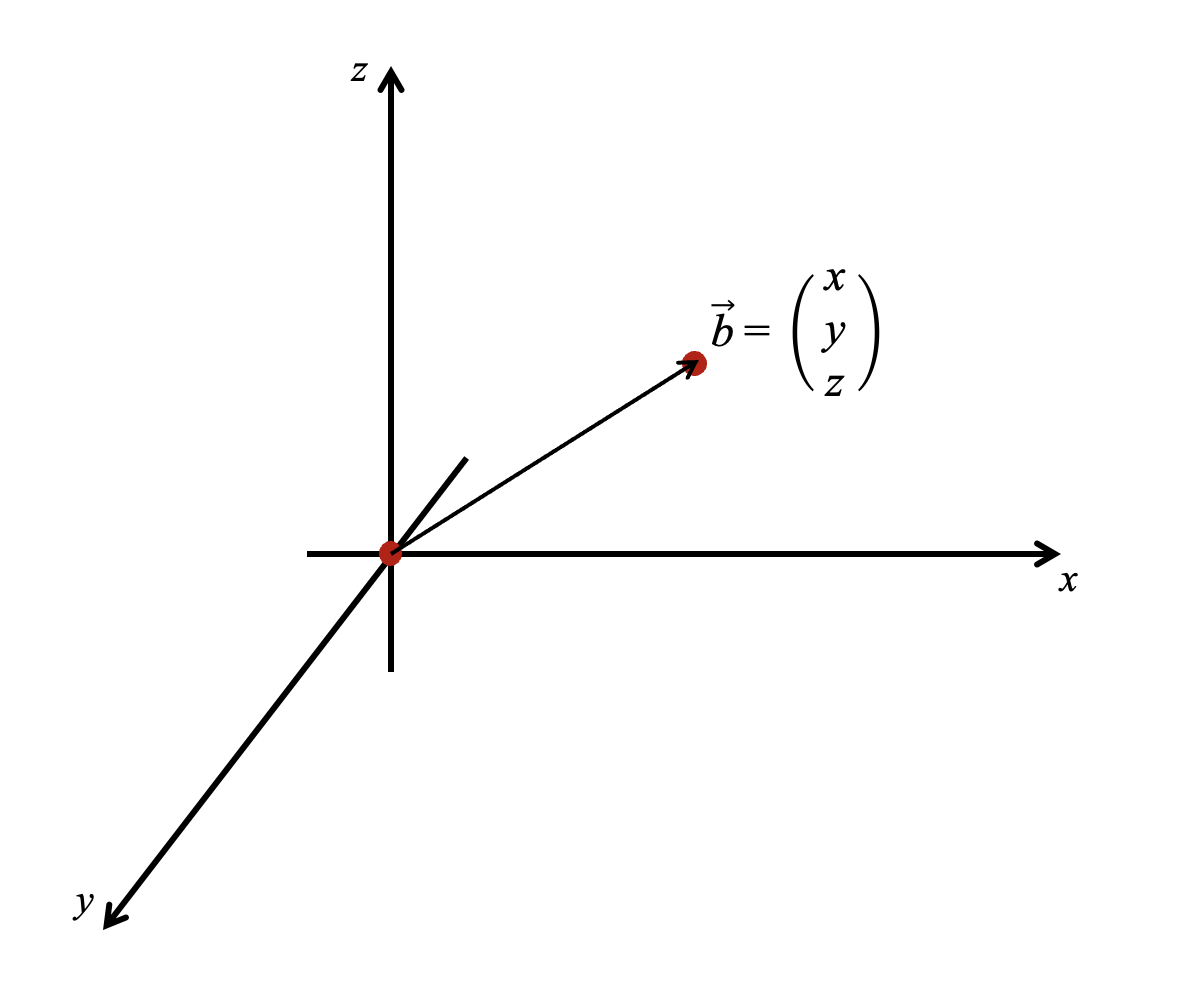
\includegraphics[width=0.5\textwidth]{Fig.2.jpg} 
            \end{figure}
            \begin{itemize}
                \item $\lim\limits_{x\rightarrow 0}\frac{1}{x}$ doest not exist. 
                $$\because \lim_{x\rightarrow 0^+}\frac{1}{x}=+\infty,\ \lim_{x\rightarrow 0^-}\frac{1}{x}=-\infty$$
                $$\therefore \lim_{x\rightarrow 0^+}\frac{1}{x}\neq\lim_{x\rightarrow 0^-}\frac{1}{x} \Rightarrow \text{DNE.} $$
                \item $\lim\limits_{x\rightarrow \infty}\frac{1}{x}$ exists. 
                $$\because \lim_{x\rightarrow +\infty}\frac{1}{x}=0,\ \lim_{x\rightarrow -\infty}\frac{1}{x}=0$$
                $$\therefore \lim_{x\rightarrow +\infty}\frac{1}{x}=\lim_{x\rightarrow -\infty}\frac{1}{x} \Rightarrow \text{Limit exists.}$$
            \end{itemize}
        \end{example}
        \begin{myclaim}{ }{}
            {\color{red}\textbf{Horizontal Asymptote (H.A.)}}: 
            $$y=\lim_{x\rightarrow \infty}f(x)=c$$
        \end{myclaim}
        \item Limit at $\infty$: 
        $${\color{red}\lim_{x\rightarrow +\infty}f(x)=\lim_{x\rightarrow -\infty}f(x)=c\ \Rightarrow \ \lim_{x\rightarrow \infty}f(x)=c}.$$
        {\color{green}{Note: $+\infty$ and $-\infty$ are not exact values; they should be regarded as a concept.}}
        \item Limites does not have to equal to the function value. \\
        Limit and the function value do not have relationships.
        \item Generally speaking, if $a \in D_f,\ \lim\limits_{x\rightarrow a}f(x)=f(a)$.
    \end{itemize}
    \item For a rational function $f(x)=\frac{P(x)}{Q(x)}$ where $P(x)=a_0x^m+a_1x^{m-1}+\cdots+a_{m-1}x+a_m$, and $Q(x)=b_0x^m+b_1x^{m-1}+\cdots+b_{m-1}x+b_m$:
    \begin{itemize}
        \item $\lim\limits_{x\rightarrow a}f(x)=f(a)\text{ as long as }Q(a)\neq 0.$
        \item $\lim\limits_{x\rightarrow \infty}f(x)=\lim\limits_{x\rightarrow \infty}\frac{a_0x^m+a_1x^{m-1}+\cdots+a_{m-1}x+a_m}{b_0x^m+b_1x^{m-1}+\cdots+b_{m-1}x+b_m}\ \Rightarrow\ \text{H.A.}$
        \begin{enumerate}
            \item If $m=n$, $\lim\limits_{x\rightarrow \infty}f(x)=\lim\limits_{x\rightarrow \infty}\frac{a_0}{b_0}=\frac{a_0}{b_0}.$
            \item If $m>n$, $\lim\limits_{x\rightarrow \infty}f(x)\text{ DNE.}$
            \item If $m<n$, $\lim\limits_{x\rightarrow \infty}f(x)=0.$
        \end{enumerate}
    \end{itemize}
    \item Continuity and Discontinuity
    \begin{myclaim}{ }{}
        \\{\color{red}\textbf{Continuity}}: If the graph of the function does not have any {\color{red}{breaks or holes}} within a certain interval, then the function is continuous within that interval.
    \end{myclaim}
    \begin{theorem}{1.1 Continuity Test}{}
        If ${\color{red}{\lim\limits_{x\rightarrow a^-}f(x)=\lim\limits_{x\rightarrow a^+}f(x)=f(a)}}$, then the function $f$ is \textbf{continuous} at $x=a$.
    \end{theorem}
\end{enumerate}

\section{Differentiation and Derivatives}
\begin{enumerate}
    \item Gradient of Secant: 
    \begin{figure}[H]
        \centering 
        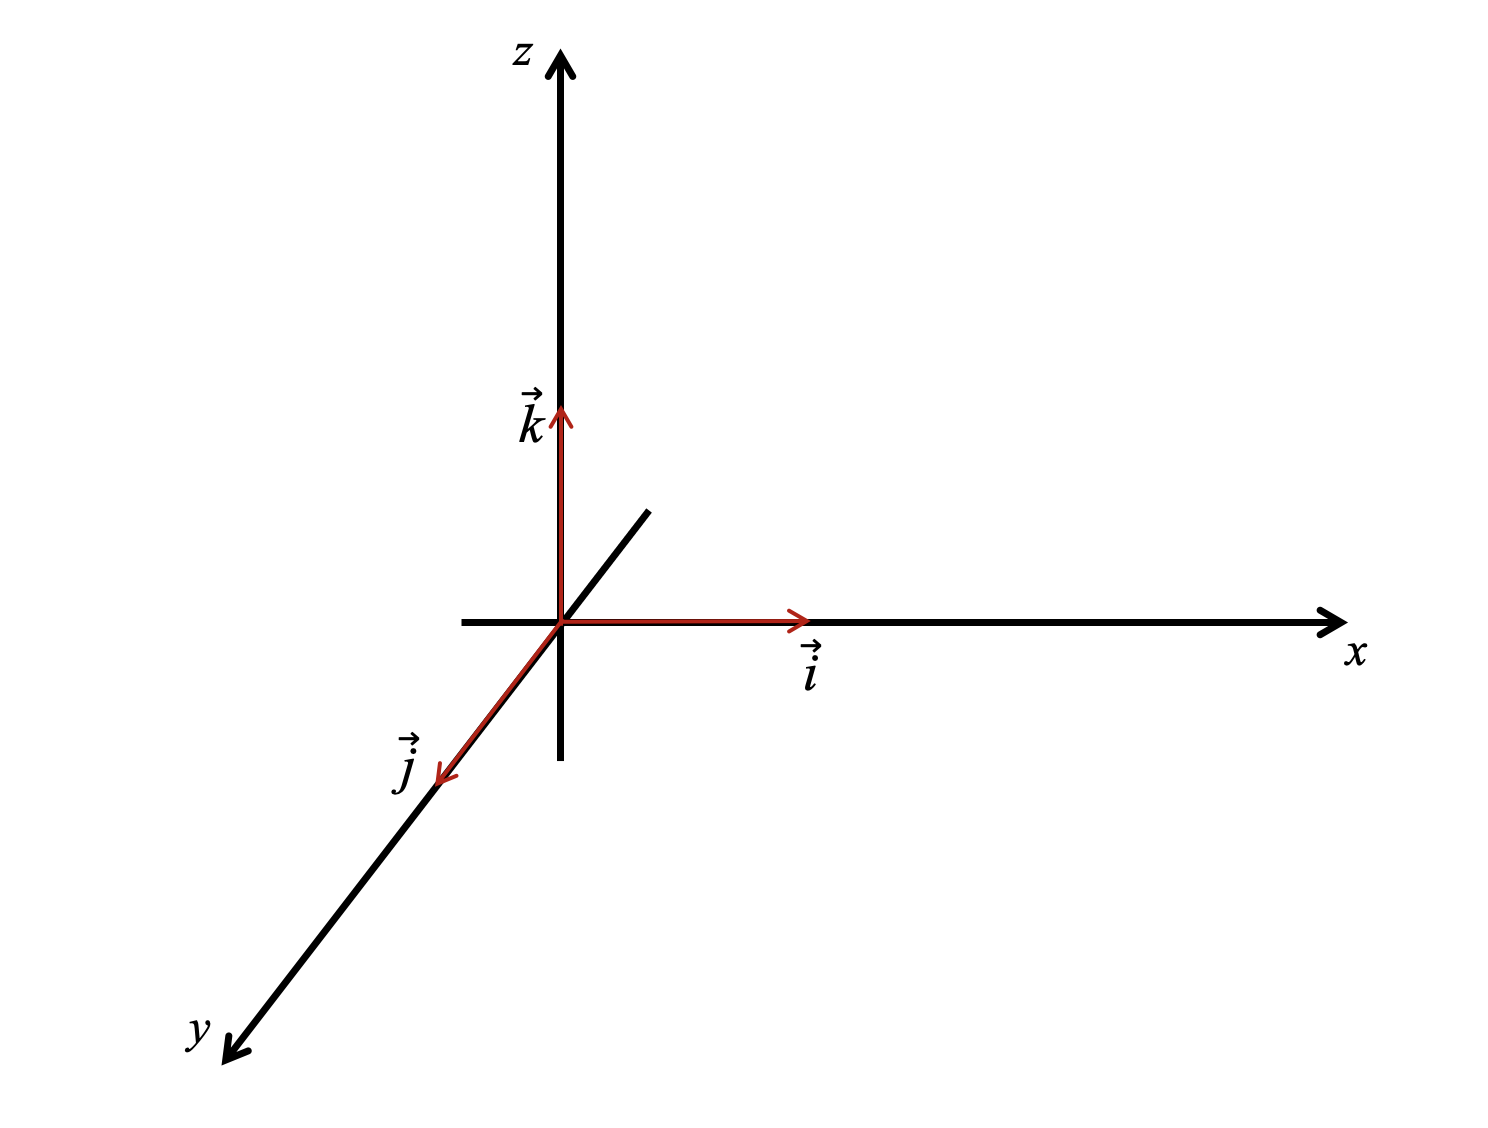
\includegraphics[width=0.5\textwidth]{Fig.3.jpg} 
    \end{figure}
    \begin{itemize}
        \item $$\text{Slope }m=\frac{f(x+\Delta x)-f(x)}{x+\Delta x-x}=\frac{f(x+\Delta x)-f(x)}{\Delta x}.$$
        \begin{myclaim}{ }{}
            \textbf{\color{red}Derivative of a function}: 
            $${\color{red}\lim_{\Delta x\rightarrow 0}\frac{f(x+\Delta x)-f(x)}{\Delta x}}\text{ is the derivative of a function, denoted as } {\color{red}\frac{\mathrm{d}y}{\mathrm{d}x}}\text{ or }{\color{red}f'(x)}.$$
        \end{myclaim}
    \item The graphic meaning of derivative is the gradient of tangent of the function. 
    \begin{example}{2.1}{}
        \textbf{By definition, find the derivative of $f(x)=x^2+1$ and hance find the gradient of the tangent line when $x=3$.}\\
        \noindent\rule[0.1pt]{\textwidth}{1pt}
        $$\begin{aligned}
            f'(x)=\lim_{x\to 0}\frac{f(x+\Delta x)-f(x)}{\Delta x}&=\lim_{x\to 0}\frac{\left[(x+\Delta x)^2+1\right]-(x^2+1)}{\Delta x}\\
            &=\lim_{x\to 0}\frac{x^2+2x\Delta x+(\Delta x)^2+1-x^2-1}{\Delta x}\\
            &=\lim_{x\to 0}\frac{2x\Delta x+(\Delta x)^2}{\Delta x}\\
            &=\lim_{x\to 0}\left(2x+\Delta x\right)\\
            &=2x.
        \end{aligned}$$
        At $x=3$, $f'(3)=2\times 3=6.$ The gradient is $6.$
    \end{example}
    \end{itemize}
    \item Derivative of $x^n$
    \begin{theorem}{2.1 Power Rule}{}
        If $f(x)=x^n$, then 
        $${\color{red}{f'(x)=nx^{n-1}}},\ \text{for any } n \in \mathbb{R}.$$
        Note: The derivative of any {\color{red}{constant}} is {\color{red}{0}}.
    \end{theorem}
    \begin{example}{2.2}{}
        $$f(x)=\frac{1}{x}=x^{-1}\ \Rightarrow\ f'(x)=(-1)x^{-1-1}=-x^{-2};$$
        $$f(x)=\sqrt{x}=x^{\frac{1}{2}}\ \Rightarrow\ f'(x)=\frac{1}{2}x^{\frac{1}{2}-1}=\frac{1}{2}x^{-\frac{1}{2}};$$
        $$f(x)=c=cx^0\ \Rightarrow\ f'(x)=0\times cx^{0-1}=0.$$
    \end{example}
    \item Rules of Differentiation: \\
    Name $f(x)$ and $g(x)$ as two functions with derivatives of $f'(x)$ and $g'(x)$, respectively.\\
    Then {\color{red}{$$\left(cf(x)\right)'=cf'(x)$$
    $$\left(f(x)\pm g(x)\right)'=f'(x)\pm g'(x)$$}}
    \item More Derivatives: 
    \begin{center}\begin{tabular}{c|c}
        $f(x)$&$f'(x)$\\ \hline
        $\sin x$&$\cos x$\\ 
        $\cos x$&$-\sin x$\\ 
        $\tan x$&$\sec^2x$\\
        $\ln x$&$\frac{1}{x}$\\
        $e^x$&$e^x$
    \end{tabular}\end{center}
    \item Differentiablity: 
    \begin{myclaim}{ }{}
        \\
        A function has to be \textbf{continuous} and \textbf{no sharp turning point} to be \textbf{\color{red}{differentiable}}.\\
        {\color{green}{Note: Smooth turning point on the graph is allowed.}}
    \end{myclaim}
    \item More Rules of Differentiation: 
    \begin{theorem}{2.2 Product Rule}{}
        Let $f(x)$ and $g(x)$ be two functions with derivatives of $f'(x)$ and $g'(x)$, respectively.
        \color{red}{$$\left(f(x)\times g(x)\right)'=f'(x)g(x)+f(x)g'(x).$$}
    \end{theorem}
    \begin{theorem}{2.3 Quotient Rule}{}
        Let $f(x)$ and $g(x)$ be two functions with derivatives of $f'(x)$ and $g'(x)$, respectively.
        \color{red}{$$\left(\frac{f(x)}{g(x)}\right)'=\frac{f'(x)g(x)-f(x)g'(x)}{g^2(x)}.$$}
    \end{theorem}
    \begin{theorem}{2.4 Chain Rule}{}
        For a composite function $f(g(x))$ or $(f\circ g)(x)$, the derivative will be $${\color{red}{f'(g(x))\times g'(x)}}.$$
        OR \\
        If $y=f(u)$ and $u=g(x)$, then $${\color{red}{\frac{\mathrm{d}y}{\mathrm{d}x}=\frac{\mathrm{d}y}{\mathrm{d}u}\cdot\frac{\mathrm{d}u}{\mathrm{d}x}}}.$$
    \end{theorem}
    \item Higher Order Differentiation: 
    $$\frac{\mathrm{d}^2y}{\mathrm{d}x^2},\ f''(x),\ f'''(x),\ f^{(4)}(x),\ f^{(5)}(x),\ \cdots$$
\end{enumerate}

\section{Applications of Derivatives}
\begin{enumerate}
    \item Equation of Tangent Line: \\
    Via the original functions, we could get the tangent point $(x_0, y_0)$. Then, the expression of the tangent line is 
    $${\color{red}{y-y_0=m(x-x_0)}},$$ 
    where $m$ is the derivative. 
    \item Normal and Tangent Lines: 
    \begin{myclaim}{ }{}
        \\\textbf{\color{red}{Normal}} is perdendicular to the tangent and passes through the same tangent point. 
        \begin{figure}[H]
            \centering 
            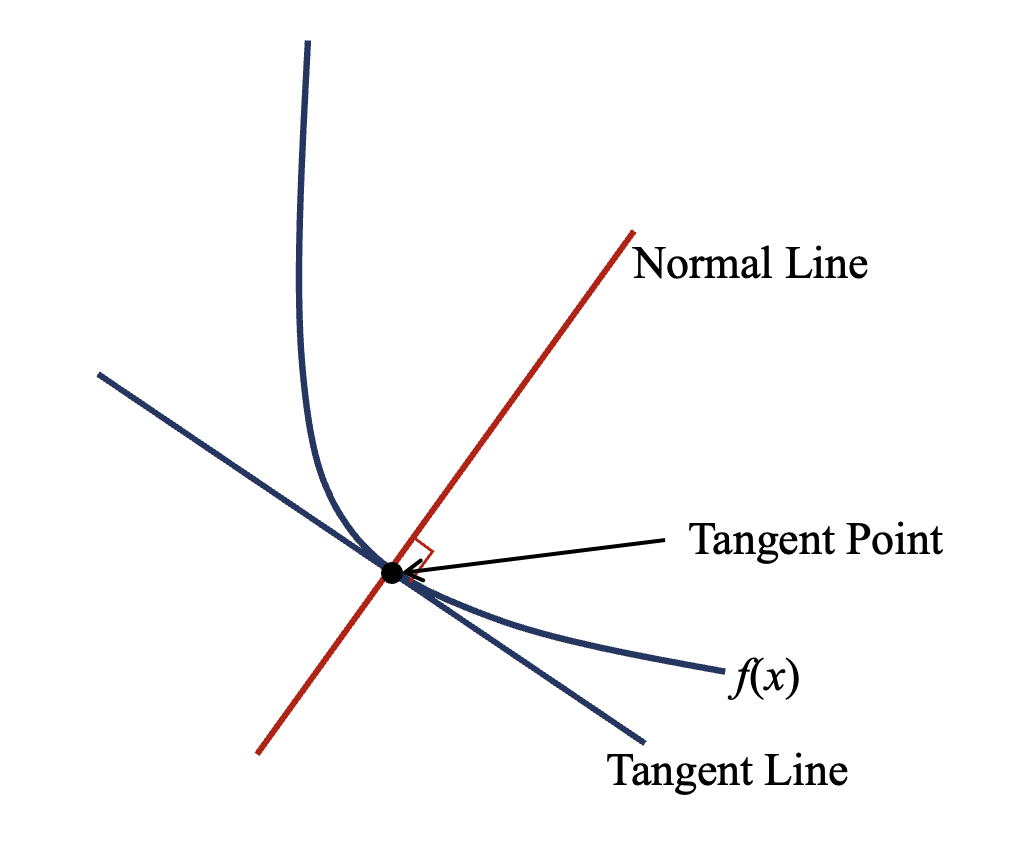
\includegraphics[width=0.5\textwidth]{Fig.4.jpg} 
        \end{figure}
    \end{myclaim}
    \item Increasing and Decreasing Function: 
    \begin{myclaim}{ }{}
        \\\textbf{\color{red}{Increasing Function}}: As $x$ is getting larger, $y$ is getting larger.\\
        i.e., $${\color{red}{\frac{\mathrm{d}y}{\mathrm{d}x}>0}}.$$
        \textbf{\color{red}{Decreasing Function}}: As $x$ is getting larger, $y$ is getting smaller.\\
        i.e., $${\color{red}{\frac{\mathrm{d}y}{\mathrm{d}x}<0}}.$$
    \end{myclaim}
    \item Local Extrema: $\color{red}{\frac{\mathrm{d}y}{\mathrm{d}x}=0}$ {\color{red}{Stationary point}}\\
    {\color{green}{Global extrema is the maximum and the minimum points of the entire function.}}\\
    $f''(x)$ is used to determine if the local extrema is maxima or minima.
    \begin{itemize}
        \item {\color{red}{Minima: $f''(x)>0$}} Concave up.
        \item {\color{red}{Maxima: $f''(x)<0$}} Concave down.
        \item {\color{red}{Point of Inflection {\color{green}{(the point that is changing from concaving up to concaving down, or vice visa)}}: $f''(x)=0$}}
    \end{itemize}
    \item With local extrema, $x$-intercepts, $y$-intercepts, concavity, and asympotes, draw approxiate diagrams of a function.
\end{enumerate}

\section{Implicit Differentiation}
\begin{enumerate}
    \item When differentiating something with $\color{red}{y}$, multiply $\color{red}{\frac{\mathrm{d}y}{\mathrm{d}x}}$ at the end. 
    \item $\color{red}{(y^2)'=2y\frac{\mathrm{d}y}{\mathrm{d}x}}$.
    \begin{proof}{4.1}{}
        If $u=y^2$, then 
        $$\frac{\mathrm{d}u}{\mathrm{d}x}=\frac{\mathrm{d}u}{\mathrm{d}y}\cdot\frac{\mathrm{d}y}{\mathrm{d}x}=2y\cdot\frac{\mathrm{d}y}{\mathrm{d}x}.\ \ \ \ \ \ \ \ \ \text{[Chain Rule]}$$
    \end{proof}
    \begin{example}{4.1}{}
        \textbf{Find $\frac{\mathrm{d}y}{\mathrm{d}x}$ for the circle $x^2+y^2=16$.}\\
        \noindent\rule[0.1pt]{\textwidth}{1pt}
        $$\begin{aligned}
            (x^2)'+(y^2)'&=(16)'\ \Rightarrow\ 2x+2y\frac{\mathrm{d}y}{\mathrm{d}x}=0\\
            \frac{\mathrm{d}y}{\mathrm{d}x}&=-\frac{2x}{2y}=-\frac{x}{y}.
        \end{aligned}$$
    \end{example}
    \begin{example}{4.2}{}
        \textbf{Find $\frac{\mathrm{d}y}{\mathrm{d}x}$ for $e^x+x\sin y=\cos 2y$.}\\
        \noindent\rule[0.1pt]{\textwidth}{1pt}
        $$\begin{aligned}
            (e^x)'+(x\sin y)'&=(\cos 2y)'\\
            e^x+\left(\sin y+x\cos y\frac{\mathrm{d}y}{\mathrm{d}x}\right)&=-2\sin 2y\frac{\mathrm{d}y}{\mathrm{d}x}\\
            (-x\cos y-2\sin 2y)\frac{\mathrm{d}y}{\mathrm{d}x}&=e^x+\sin y\\
            \frac{\mathrm{d}y}{\mathrm{d}x}&=\frac{e^x+\sin y}{-x\cos y-2\sin 2y}.
        \end{aligned}$$
    \end{example}
    \item Second Order Differentiation of Implicit functions*: Differentiate the first order differentiation.
    \begin{example}{4.3}{}
        \textbf{Find $\frac{\mathrm{d}^2y}{\mathrm{d}x^2}$ for the circle $x^2+y^2=16$.} (From Ex. 4.1: $2x+2y\frac{\mathrm{d}y}{\mathrm{d}x}=0,\ \frac{\mathrm{d}y}{\mathrm{d}x}=-\frac{2x}{2y}=-\frac{x}{y}.$)\\
        \noindent\rule[0.1pt]{\textwidth}{1pt}
        $$(2x)'+\left(2y\frac{\mathrm{d}y}{\mathrm{d}x}\right)'=(0)'\Rightarrow2+\left((2y)'\frac{\mathrm{d}y}{\mathrm{d}x}+2y\left(\frac{\mathrm{d}y}{\mathrm{d}x}\right)'\right)=0\Rightarrow2+2\left(\frac{\mathrm{d}y}{\mathrm{d}x}\right)^2+2y\frac{\mathrm{d}^2y}{\mathrm{d}x^2}=0$$
        $$\frac{\mathrm{d}^2y}{\mathrm{d}x^2}=\frac{-2-2\left(\frac{\mathrm{d}y}{\mathrm{d}x}\right)^2}{2y}=\frac{-2-2\left(-\frac{x}{y}\right)^2}{2y}.$$
    \end{example}
    \item Derivative of Inverse Trignometry Functions
    \begin{theorem}{4.1}{}
        $$y=\arcsin x\ \Rightarrow\ {\color{red}{\frac{\mathrm{d}y}{\mathrm{d}x}}=\frac{1}{\cos y}=\frac{1}{\sqrt{1-x^2}}},\ \arcsin x\in\left[-\frac{\pi}{2},\frac{\pi}{2}\right](\cos y>0).$$
        \begin{proof}{4.1}{}
            From $y=\arcsin x,$ we get $\sin y=x$. This situation can be illustrated by the figure below: 
            \begin{figure}[H]
                \centering 
                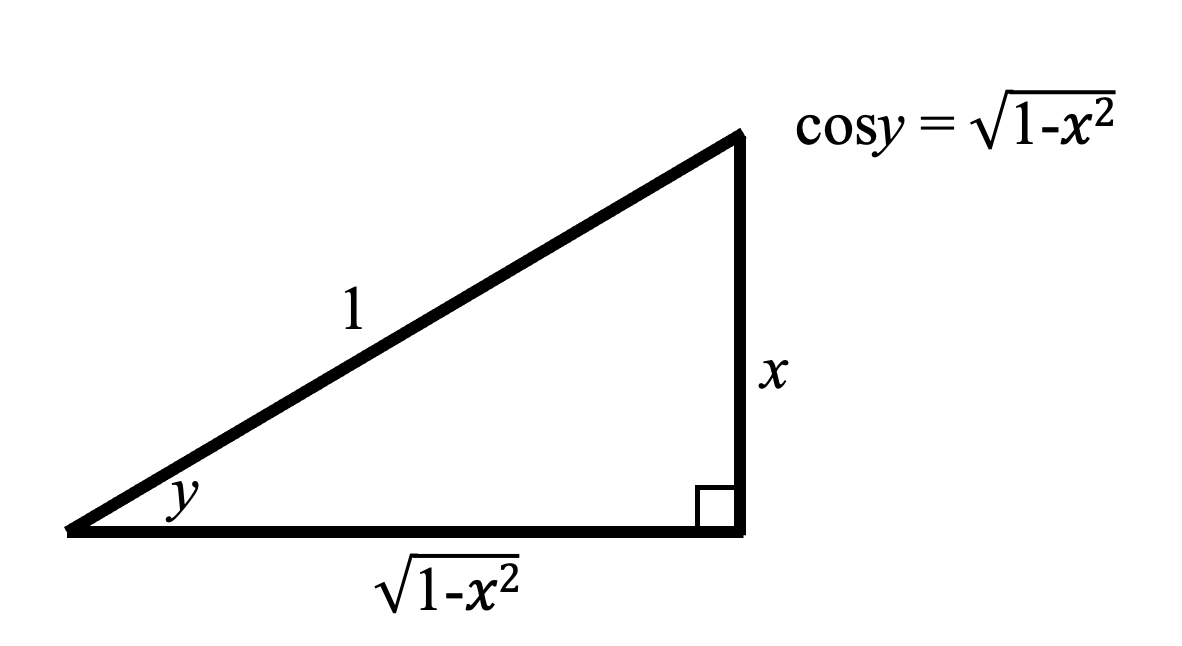
\includegraphics[width=0.5\textwidth]{Fig.5.jpg} 
            \end{figure}
            $$\therefore (\sin y)'=(x)'\ \Rightarrow\ \cos y\frac{\mathrm{d}y}{\mathrm{d}x}=1$$
            $$\therefore \frac{\mathrm{d}y}{\mathrm{d}x}=\frac{1}{\cos y}=\frac{1}{\sqrt{1-x^2}}.$$
        \end{proof}
    \end{theorem}
    \begin{theorem}{4.2}{}
        $$y=\arccos x\ \Rightarrow\ {\color{red}{\frac{\mathrm{d}y}{\mathrm{d}x}}=-\frac{1}{\sin y}=-\frac{1}{\sqrt{1-x^2}}},\ \arccos x\in\left[0,\pi\right](\sin y>0).$$
        $$y=\arctan x\ \Rightarrow\ {\color{red}{\frac{\mathrm{d}y}{\mathrm{d}x}}=\frac{1}{1+x^2}}.$$
        \begin{proof}{4.2}{}
            {\color{green}{(Hint: Try to visualize a similar diagram as in proof 4.1.)}}\\
            From $y=\arccos x,$ we get $\cos y=x$. 
            $$\therefore (\cos y)'=(x)'\ \Rightarrow\ -\sin y\frac{\mathrm{d}y}{\mathrm{d}x}=1\ \Rightarrow\ \frac{\mathrm{d}y}{\mathrm{d}x}=-\frac{1}{\sin y}=-\frac{1}{\sqrt{1-x^2}}.$$
            From $y=\arctan x,$ we get $\tan y=x$.
            $$\therefore (\tan y)'=(x)'\Rightarrow\sec^2 y\frac{\mathrm{d}y}{\mathrm{d}x}=1\Rightarrow\frac{\mathrm{d}y}{\mathrm{d}x}=\frac{1}{\sec^2 y}=\cos^2 y=\left(\frac{1}{\sqrt{1+x^2}}\right)=\frac{1}{1+x^2}.$$
        \end{proof}
    \end{theorem}
\end{enumerate}

\section{Related Rate of Change}
\begin{enumerate}
    \item When finding a rate of change of $x$, we are finding the $\frac{\mathrm{d}y}{\mathrm{d}x}$.
    \begin{example}{5.1}{}
        \textbf{Area of circle is increasing at a rate of $10\pi$ per second. When the raduis is $2$, what is the rate of change of radius? }\\
        \noindent\rule[0.1pt]{\textwidth}{1pt}
        Known: $\frac{\mathrm{d}A}{\mathrm{d}t}=10\pi,\ r=2$. Find: $\frac{\mathrm{d}r}{\mathrm{d}t}$.
        $$\begin{aligned}
            A=\pi r^2 \ \Rightarrow \ \frac{\mathrm{d}A}{\mathrm{d}t}=2\pi r\frac{\mathrm{d}r}{\mathrm{d}t}&=10\pi\\
            \frac{\mathrm{d}r}{\mathrm{d}t}&=\frac{10\pi}{2\pi r}=\frac{5}{r}
        \end{aligned}$$
        $$\text{When }r=2,\ \frac{\mathrm{d}r}{\mathrm{d}t}=\frac{5}{2}.$$
    \end{example}
    \begin{example}{5.2}{}
        \textbf{A spherical balloon is expanding at a rate of $60\pi$ per second. How fast is the surface area of the balloon expanding when the radius is $4$? }\\
        \noindent\rule[0.1pt]{\textwidth}{1pt}
        Known: $\frac{\mathrm{d}V}{\mathrm{d}t}=60\pi,\ r=4$. Find $\frac{\mathrm{d}A}{\mathrm{d}t}$.
        $$\begin{aligned}
            V=\frac{4}{3}\pi r^3\ \Rightarrow\ \frac{\mathrm{d}V}{\mathrm{d}t}=3\cdot\frac{4}{3}\pi r^2\frac{\mathrm{d}r}{\mathrm{d}t}&=4\pi r^2\frac{\mathrm{d}r}{\mathrm{d}t}\\
            \therefore 4\pi r^2\frac{\mathrm{d}r}{\mathrm{d}t}=60\pi\ &\Rightarrow\ \frac{\mathrm{d}r}{\mathrm{d}t}=\frac{60\pi}{4\pi r^2}=\frac{15}{r^2}\\
            A=4\pi r^2\ \Rightarrow\ \frac{\mathrm{d}A}{\mathrm{d}t}=8\pi r\frac{\mathrm{d}r}{\mathrm{d}t}=8&\pi r\cdot\frac{15}{r^2}=\frac{120\pi}{r}.
        \end{aligned}$$
        $$\text{When }r=4,\ \frac{\mathrm{d}A}{\mathrm{d}t}=\frac{120\pi}{4}=30\pi.$$
    \end{example}
    \item Kinematics: 
    \begin{itemize}
        \item {\color{red}{Velocity}}, {\color{red}{displacement}}, and {\color{red}{acceleration}} are vector variables that have a value and a direction. 
        \item {\color{red}{Speed}} only has a value and no direction. It is a scalar variable. {\color{green}{No sign should be reported in the answer}}.
        \item If $s$ is the displacement, $v$ is the velocity, $a$ is the acceleration: $${\color{red}{\frac{\mathrm{d}s}{\mathrm{d}t}=v}};\ {\color{red}{\frac{\mathrm{d}v}{\mathrm{d}t}=a}}.$$
    \end{itemize}
\end{enumerate}

\section{More Limits - L'Hopital's Rule}
\begin{theorem}{6.1 L'Hopital's Rule}{}
    When the limit is in the \textbf{\color{red}{indeterminant form}} ($\frac{0}{0}$ or $\frac{\infty}{\infty}$), 
    $${\color{red}{\lim_{x\rightarrow a}\left[\frac{f(x)}{g(x)}\right]\lim_{x\rightarrow a}\left[\frac{f'(x)}{g'(x)}\right]}},$$
    where $f'(x)$ and $g'(x)$ are the first derivatives of $f(x)$ and $g(x)$, respectively. 
\end{theorem}
\begin{example}{6.1}{}
    $$\lim_{x\rightarrow 0}\frac{\tan x}{x}=\lim_{x\rightarrow 0}\frac{\sec^2x}{1}=1$$
\end{example}

\section{Indefinite Integration}
\begin{enumerate}
    \item Regard Integration as Anti-differentiation: 
    $$f'(x)=x\ \ \ \Rightarrow\ \ \ f(x)=\frac{1}{2}x^2+C,\ \text{where }C\text{ is a constant.}$$
    $$f'(x)=x^2\ \ \ \Rightarrow\ \ \ f(x)=\frac{1}{3}x^3+C,\ \text{where }C\text{ is a constant.}$$
    $$f'(x)=x^n\ \ \ \Rightarrow\ \ \ f(x)=\frac{1}{n+1}x^{n+1}+C,\ \text{where }C\text{ is a constant.}$$
    \begin{myclaim}{ }{}
        \\Anti-differentiation is also called \textbf{\color{red}{indefinited integration}}. It is denoted by {\color{red}{$\int \ \mathrm{d}x.$}}
        \begin{center}{\color{green}{e.g. $\int x^n\ \mathrm{d}x=\frac{1}{n+1}x^{n+1}+C.$}}\end{center}
    \end{myclaim}
    \item General Rules of Integration. 
    \begin{itemize}
        \item $${\color{red}{\int x^n\ \mathrm{d}x=\frac{1}{n+1}x^{n+1}+C}}$$
        \item $${\color{red}{\int k\ \mathrm{d}x=kx+C}}$$
        \item $${\color{red}{\int kf(x)\ \mathrm{d}x=k\int f(x)\ \mathrm{d}x}}$$
        \item $${\color{red}{\int f(x)\pm g(x)\ \mathrm{d}x=\int f(x)\ \mathrm{d}x\pm\int g(x)\ \mathrm{d}x}}$$
    \end{itemize}
    \item $\int f'(x)\ \mathrm{d}x=f(x)+C.$ Therefore, if we know the $f'(x)$ and a point on the $f(x)$, which is to determine the constant $C$, then we can deduce the original function $f(x)$.
    \item More Rules of Integration:
    \begin{center}\begin{tabular}{c|c}
        Differentiation&Integration\\\hline
        $(e^x)'=e^x$&${\color{red}{\int e^x\ \mathrm{d}x}=e^x+C}$\\
        $(\ln x)'=frac{1}{x}$&${\color{red}{\int \frac{1}{x}\ \mathrm{d}x}=\ln x+C}$\\
        $(\sin x)'=\cos x$&${\color{red}{\int \cos x\ \mathrm{d}x}=\sin x+C}$\\
        $(\cos x)'=-\sin x$&${\color{red}{\int \sin x\ \mathrm{d}x}=-\cos x+C}$\\
        $(\tan x)'=\sec^2 x$&${\color{red}{\int \sec^2 x\ \mathrm{d}x}=\tan x+C}$\\
        $(\cot x)'=-\csc^2 x$&${\color{red}{\int \csc^2 x\ \mathrm{d}x}=-\cot x+C}$\\
        $(\sec x)'=\sec x\tan x$&${\color{red}{\int \sec x\tan x\ \mathrm{d}x}=\sec x+C}$\\
        $(\csc x)'=-\csc x\cot x$&${\color{red}{\int \csc x\cot x\ \mathrm{d}x}=-\csc x+C}$\\
    \end{tabular}\end{center}
    \item Anti-chain Rule in Integration: We must {\color{red}{divide}} the chain rule factor.
    \begin{example}{7.1}{}
        $$\int (ax+b)^n\ \mathrm{d}x=\frac{1}{a}\left(\frac{1}{n+1}(ax+b)^{n+1}\right)+C$$
        $$\int e^{(ax+b)}\ \mathrm{d}x=\frac{1}{a}e^{ax+b}+C$$
        $$\int \frac{1}{(ax+b)}\ \mathrm{d}x=\frac{1}{a}\ln(ax+b)+C$$
        $$\int \sin{(ax+b)}\ \mathrm{d}x=-\frac{1}{a}\cos(ax+b)+C$$
        $$\int \cos{(ax+b)}\ \mathrm{d}x=\frac{1}{a}\sin(ax+b)+C$$
    \end{example}
    \item Integration Techniques: by Substitution and by Parts: 
    \begin{theorem}{7.1 Integration By Substitution}{}
        Whenever we have an integration like: $\int g'(x)\times f(g(x))\ \mathrm{d}x$, we can always assume {\color{red}{$u=g(x)$}}. Therefore, $\mathrm{d}u=g'(x)\cdot\mathrm{d}x$. {\color{green}{()$u=g(x)\ \Rightarrow\ \frac{\mathrm{d}u}{\mathrm{d}x}=g'(x)$)}}: 
        $${\color{red}{\int g'(x)\times f(g(x))\ \mathrm{d}x=\int f(u\ \mathrm{d}u)}}.$$
    \end{theorem}
    \begin{theorem}{7.2 Integration By Parts}{}
        If $f(x)$ and $g(x)$ are two functions, and $f'(x)$ and $g'(x)$ are their derivatives, respectively, integration by parts can be written as following:         $${\color{red}{\int f(x)g'(x)\ \mathrm{d}x=f(x)g(x)-\int f'(x)g(x)\ \mathrm{d}x}}.$$
    \end{theorem}
    \begin{example}{7.2}{}
        \textbf{Find $\int 2x(x^2+3)^5\ \mathrm{d}x$.}\\
        \noindent\rule[0.1pt]{\textwidth}{1pt}
        Since $2x=(x^2+3)'$, we consider to use integration by substitution. \\
        Assume $u=x^2+3$, then $\frac{\mathrm{d}u}{\mathrm{d}x}=(x^2+3)'=2x\ \Rightarrow\ \mathrm{d}u=2x\cdot \mathrm{d}x.$
        $$\begin{aligned}
            \therefore\int 2x(x^2+3)^5\ \mathrm{d}x&=\int (x^2+3)^5\cdot (2x\cdot\mathrm{d}x)\\
            &=\int u^5\ \mathrm{d}u\\
            &=\frac{1}{6}u^6+C\\
            &=\frac{1}{6}(x^2+3)^6+C.
        \end{aligned}$$
    \end{example}
    \item Integration of Inverse Trignometric Functions: 
    \begin{itemize}
        \item $${\color{red}{\int \frac{1}{\sqrt{1-x^2}}\ \mathrm{d}x=\arcsin x+C}}$$
        \item $${\color{red}{\int \frac{1}{1+x^2}\ \mathrm{d}x=\arctan x+C}}$$
        \item $${\color{red}{\int \frac{1}{x\sqrt{x^2-1}}\ \mathrm{d}x=\text{arcsec} x+C}}$$
    \end{itemize}
    \begin{example}{7.3}{}
        \textbf{Find $\int \frac{\mathrm{d}x}{x^2+4x+5}$}\\
        \noindent\rule[0.1pt]{\textwidth}{1pt}
        $$\begin{aligned}
            \int \frac{\mathrm{d}x}{x^2+4x+5}&=\frac{\mathrm{d}x}{(x+2)^2+1}\\
            \text{Assume }u&=x+2,\ \frac{\mathrm{d}u}{\mathrm{d}x}=1\ \Rightarrow\ \mathrm{d}u=\mathrm{d}x\\
            \therefore  \int \frac{\mathrm{d}x}{x^2+4x+5}&=\frac{\mathrm{d}u}{u^2+1}\\
            &=\arctan u+C\\
            &=\arctan (x+2)+C.
        \end{aligned}$$
    \end{example}
\end{enumerate}

\section{Approximiating the Area Under a Curve}
\begin{enumerate}
    \item The {\color{red}{definite integral}} is equal to the limit at infinity of the Riemann sum, and hence gives the exact area under the curve between $x=a$ and $x=b$. i.e., 
    $${\color{red}{\lim_{n\to\infty}=\sum_{i}^{n}f(x_i)\Delta x_i=\int_a^b f(x)\ \mathrm{d}x}}, $$
    where $a$ is the lower limit and $b$ is the upper limit. 
    \item If $f(x)\geq 0\ \forall x\in\left[a,b\right]$, then $\int_a^bf(x)\ \mathrm{d}x$ is defined as the shaded area: 
    \begin{figure}[H]
        \centering 
        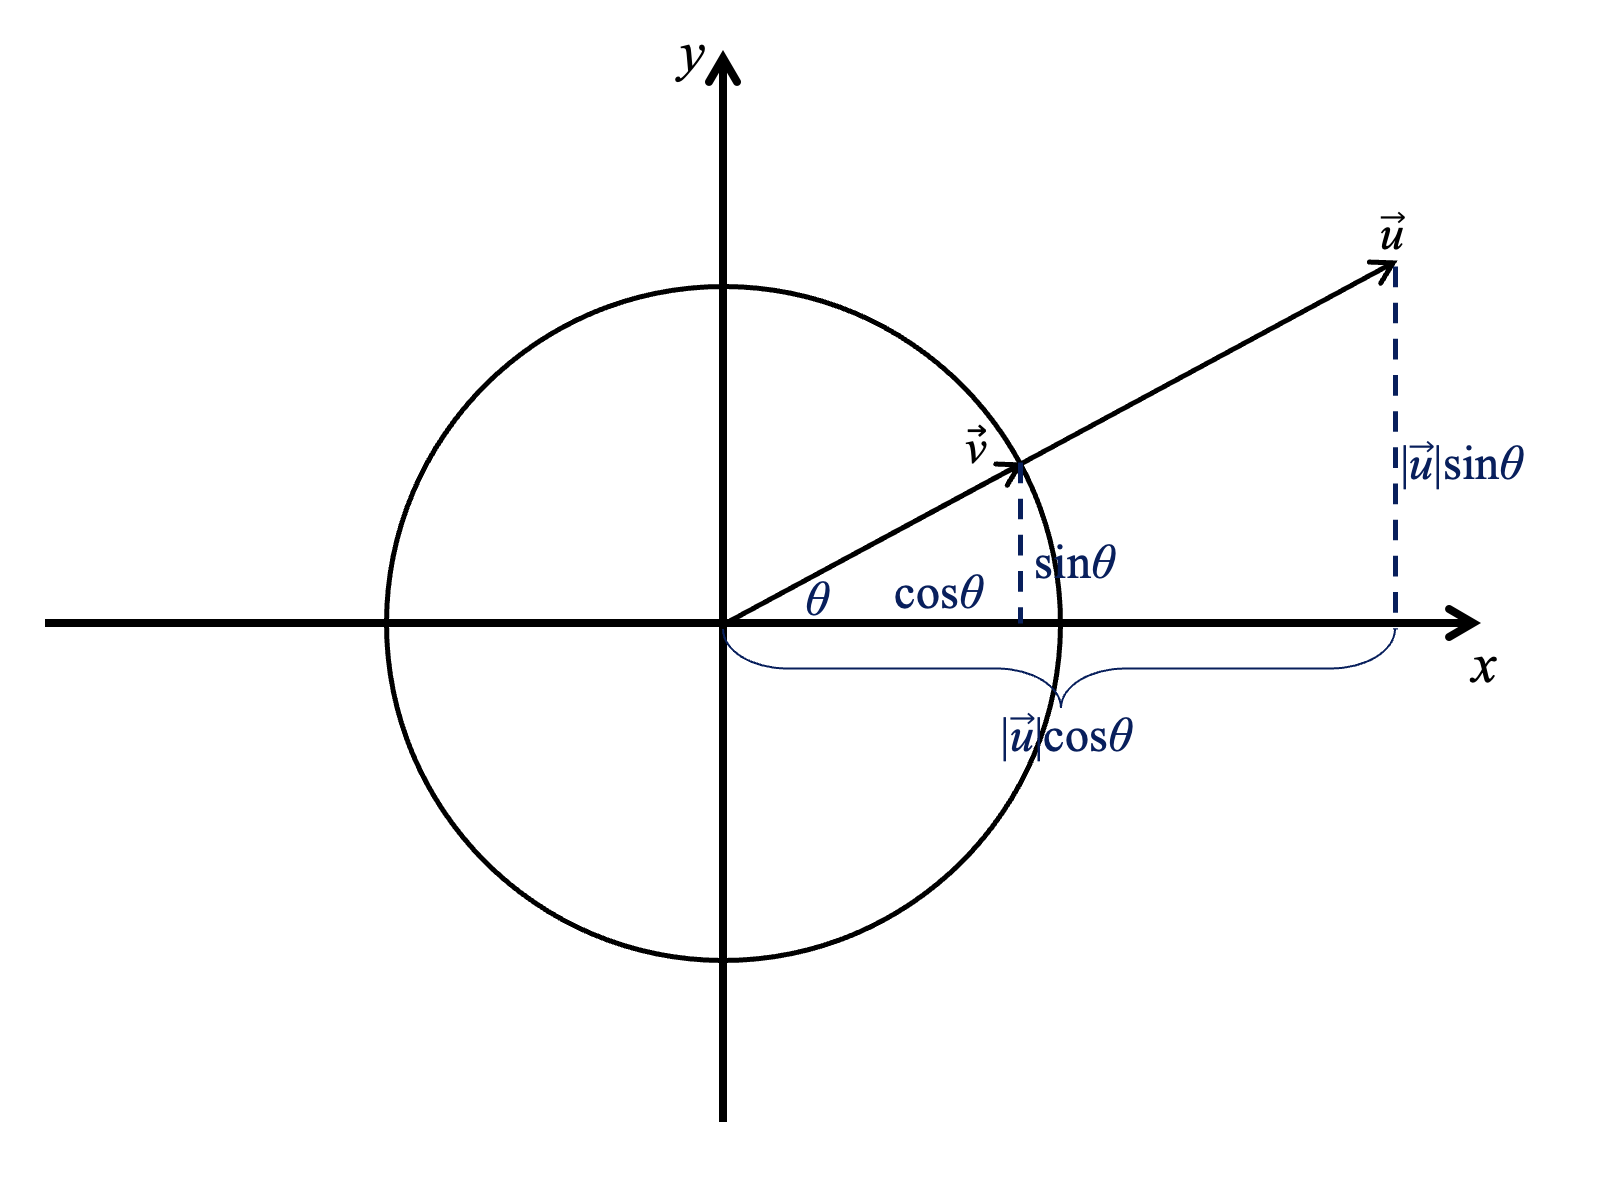
\includegraphics[width=0.5\textwidth]{Fig.6.jpg} 
    \end{figure}
    This is known as the {\color{red}{Riemann integral}}.
    \item The {\color{red}{Fundamental Theorem of Calculus}}: 
    \begin{theorem}{8.1 Fundamental Theorem of Calculus}{}
        For a continuous function $f(x)$ with antiderivative $F(x)$: 
        $${\color{red}{\int_a^bf(x)\ \d x=F(b)-F(a)}}.$$
        This theorem explains the link between differential calculus and the definite integral. 
    \end{theorem}
    \item Properties of Definite Integrals: 
    \begin{itemize}
        \item $$\int_a^af(x)\ \d x=0$$
        \item $$\int_a^bd\ \d x=k(b-a),\ (k\text{ is a constant}).$$
        \item $$\int_b^af(x)\ \d x=-\int_a^bf(x)\ \d x$$
        \item $$\int_a^bkf(x)\ \d x=k\int_a^bf(x)\ \d x$$
        \item $$\int_a^bf(x)\ \d x+\int_b^cf(x)\ \d x=\int_a^cf(x)\ \d x$$
        \item $$\int_a^b\left[f(x)\pm g(x)\right]\ \d x=\int_a^bf(x)\ \d x\pm\int_a^bg(x)\ \d x$$
    \end{itemize}
    \item When the function $f(x)$ is {\color{red}{negative}} for $x\in\left[a,b\right]$, then the area bounded by the curve, the $x$-axis and the lines $x=a$ and $x=b$ is given by 
    $${\color{red}{\left|\int_a^bf(x)\ \d x\right|}}.$$
    \item Finding Areas Between Two Functions: 
    \begin{itemize}
        \item Sketch: find the intersections and determine which function is above.
        \item Integration.
    \end{itemize}
\end{enumerate}

\section{Volumes of Revolution}
\begin{enumerate}
    \item The volume of a solid of revolution formed when $y=f(x)$, which is continuous in the interval $\left[a,b\right]$, is rotated $2\pi$ radians about the $x$-axis is given by 
    $${\color{red}{V=\pi\int_a^by^2\ \d x}}.$$
    \item The volume of a solid of revolution formed when $y=f(x)$, which is continuous in the interval $y=c$ to $y=d$, is rotated $2\pi$ radians about the $y$-axis is given by
    $${\color{red}{V=\pi\int_c^dx^2\ \d y}}.$$
    \item Consider a region $R$ between two curves, $y=f(x)$ and $y=g(x)$, from $x=a$ to $x=b$, when $f(x)>g(x)$.
    \begin{figure}[htbp]
        \centering
        \subfigure[]{
            \begin{minipage}[t]{0.25\linewidth}
            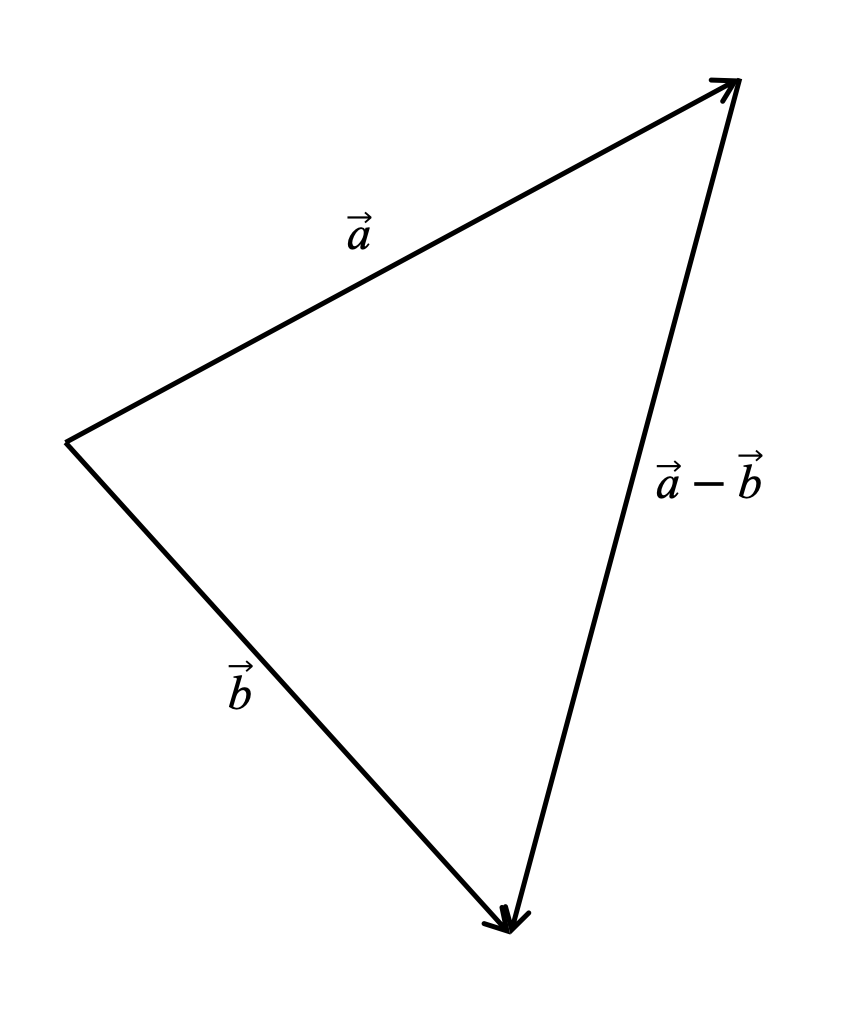
\includegraphics[width=2.1in]{Fig.7.jpg}
            \end{minipage}}
        \subfigure[]{
        \begin{minipage}[t]{0.25\linewidth}
        \includegraphics[width=1.55in]{Fig.8.jpg}
        \end{minipage}}
    \end{figure}
    \begin{itemize}
        \item Rotating $R$ about the $x$-axis generates a solid of revolution $S$. 
        The criss-section of this shape looks like a washer whose area is given by: $$A=\pi(R^2-r^2)=\pi\left(\left(f(x)\right)^2-\left(g(x)\right)^2\right).$$
        So the volume of $S$ is given by: 
        $$\begin{aligned}
            V&=\int_a^bA(x)\ \d x\\
            &={\color{red}{\int_a^b\left((f(x))^2-(g(x))^2\right)\ \d x}}.
        \end{aligned}$$
        \item Rotating $R$ about the $y$-axis in the interval $c\leq y\leq d$: 
        $${\color{red}{V=\pi\int_c^d\left((x_1)^2-(x_2)^2\right)\ \d y}},$$
        where $x_1$ and $x_2$ are expression of $x$ with respect to $y$ of $f(x)$ and $g(x)$.
    \end{itemize}
\end{enumerate}

\section{Differential Equation}
\begin{enumerate}
    \item Differential Equation: 
    \begin{myclaim}{ }{}
        \\A \textbf{\color{red}{differential equation}} is an equation containing the derivatives of one or more dependent variables with respect to one or more independent variables. {\color{green}{Equation that involves the derivatives of one or more functions}}.
    \end{myclaim}
    {\color{green}{E.g. $$y'=6x+1\ \ \ \ \ \ \text{Lagrage notation}$$$$3\frac{\d^2y}{\d x^2}+5\frac{\d y}{d x}-y=3\ \ \ \ \ \ \text{Leibriz notation}$$$$f'(x)=6x+1\ \ \ \ \ \ \text{Function notation}$$}}
    The independent variable is $x$, and the dependent variable is $y$. The solution to a differential equation is a function or a set of functions. 
    \item Two Types of Differential Equations: 
    \begin{myclaim}{ }{}
        \\\textbf{\color{red}{Ordinary Differential Equations (ODEs)}}: deals with functions of a single variable and ordinary derivatives. 
        \\\textbf{\color{red}{Partial Differential Equations (PDEs)}}: deals with multivariable equations and their partial derivatives (with more than one independent variables).
    \end{myclaim}
    \item Order of Differential Equations: 
    \begin{myclaim}{ }{}
        \\The \textbf{\color{red}{order of the differential equation}} is the highest order derivative in the equation. 
    \end{myclaim}
    \item Linearity of ODEs: 
    \begin{theorem}{10.1}{}
        A differential equation is said to be \textbf{\color{red}{linear}} if: 
        \begin{itemize}
            \item All the terms with dependent variabels are in first-order.
            \item The coefficients of all the terms in the dependent variable and its derivatives depend only on the independent variable $x$.
        \end{itemize}
    \end{theorem}
    \item Linear First-Order ODEs: 
    \begin{myclaim}{ }{}
        $${\color{red}{\frac{\d y}{\d x}+a(x)y=b(x)}},\text{ where }a(x)\text{ and }b(x)\text{ are functions of }x.$$
    \end{myclaim}
    \item Solutions of ODEs: 
    \begin{itemize}
        \item The solution to an ODE is a function or a set of functions.
        \item {\color{red}{General solution}} to the differential equation: \\
        For a differential equation of order $n$, a solution is a function that satisfies the equation on some interval $I$. The function should havee at least its first $n$ derivatives on this invertal $I$. 
        \item To find {\color{red}{particular solutions}}, we need to initial conditions for the problem. 
        \begin{enumerate}
            \item {\color{red}{Initial Value Problem (IVP)}}: where initial values are given to solve the differential equations depending on the order of the ODE. \\
            {\color{green}{E.g. $y(0),\ t(0),\ (0,y)$.}}
            \item {\color{red}{Boundary Value Problem}}: where a certain boundary is given. \\
            {\color{green}{E.g. $(x,y)$.}}
        \end{enumerate}
    \end{itemize}
    \item Separable Differential Equations: 
    \begin{myclaim}{ }{}
        \\A differential equation $\frac{\d y}{\d x}=f(x,y)$ is \textbf{\color{red}{separable}} if it can be expressed as a product of a function in $x$ and a function in $y$: 
        $${\color{red}{\frac{\d y}{\d x}=f(x,y)=g(x)h(y)}}.$$
    \end{myclaim}
    \begin{itemize}
        \item Particularly, if $h(x)\neq 0$, the variable can be separated to 
        $$\color{red}\begin{aligned}
            {\frac{\d y}{\d x}=g(x)h(y)}\ \Rightarrow \frac{\d y}{h(y)}&=g(x)\ \d x\\
            \int \frac{\d y}{h(y)}&=\int g(x)\ \d x
        \end{aligned}$$
        \item Solving differential equations using separation of variables: 
        \begin{enumerate}
            \item Separate the variables such that everything involving $y$ is on one side and everything involving $x$ is on the other side. 
            \item Integrate both sides and combine the constant of integration on one side of the equation (normally the right side).
        \end{enumerate}
        \begin{example}{10.1}{}
            \textbf{Solve for $y$ if $\frac{\d y}{\d x}=x(1+y)e^x$.}\\
            \noindent\rule[0.1pt]{\textwidth}{1pt}
            $$\begin{aligned}
                \frac{\d y}{\d x}&=x(1+y)e^x\\
                \frac{1}{1+y}\d y&=xe^x\d x\\
                \int \frac{1}{1+y}\ \d y&=\int xe^x\ \d x\\
                {\color{green}{(=xe^x-\int e^x\ \d x}}&{\color{green}{=xe^x-e^x\ \text{[Integration by Parts]})}}\\
                \ln{|1+y|}&=xe^x-e^x+C\\
                1+y&=e^{xe^x-e^x+C}=e^{xe^x-e^x}\cdot e^C\\
                y&=Ae^{xe^x-e^x}-1\ \ \ (A=e^{C}).
            \end{aligned}$$
        \end{example}
    \end{itemize}
    \item The Standard Logistic Equation: 
    $${\color{red}{\frac{\d u}{\d t}=kn(a-n);\ \ a,k\in \R}}.$$
    where $t$ is the time during which a population grows, \\
        $n$ is the population after time $t$, \\
        $k$ is the relative growth, and \\
        $a$ is a constant. 
    \item Homogeneous Differential Equations: 
    \begin{myclaim}{ }{}
        \\Differential equations of the form $\frac{\d y}{\d x}=f\left(\frac{y}{x}\right)$, where $y=y(x)$, are known as \textbf{\color{red}{homogeneous differential equations}}.
    \end{myclaim}
    \begin{theorem}{10.2}{}
        Homogeneous differential equations can be solved by using the substituion \textbf{\color{red}{$y=vx$}}, where $v$ is a function of $x$. The substitution will always reduce the differential equation to a separable differential equation. 
        \begin{proof}{Theorem 10.2}{}
            If $y=vx$, where $v$ is a function of $x$, then: 
            $$\begin{aligned}
                \frac{\d y}{\d x}&=\frac{\d v}{\d x}x+v\ \ \ \ \ \ \text{[Product Rule]}\\
                \because \frac{\d y}{\d x}&=f\left(\frac{y}{x}\right),\\
                \therefore \frac{\d v}{\d x}x+v&=f\left(\frac{y}{x}\right)=f(v)\\
                \frac{\d v}{\d x}&=\frac{f(v)-v}{x}\\
                \Rightarrow \frac{1}{f(v)-v}\ \d v&=\frac{1}{x}\ \d x
            \end{aligned}$$
        \end{proof}
    \end{theorem}
    \begin{example}{10.2}{}
        \textbf{Solve for $\frac{\d y}{\d x}=\frac{x+2y}{x}$, given $y(3)=\frac{3}{2}$.}\\
        \noindent\rule[0.1pt]{\textwidth}{1pt}
        $$\frac{\d y}{\d x}=1+2\frac{y}{x}\ \rightarrow\ \text{homogenous differential equation}$$
        $$\text{Let }y=vx,\ \frac{\d y}{\d x}=\frac{\d v}{\d x}x+v\ \Rightarrow\ \frac{\d v}{\d x}x+v=1+2\frac{y}{x}=1+2v.$$
        $$\begin{aligned}
            \frac{\d v}{\d x}&=\frac{1+v}{x}\\
            \frac{1}{1+v}\ \d v&=\frac{1}{x}\ \d x\\
            \int \frac{1}{1+v}\ \d v&=\int \frac{1}{x}\ \d x\\
            \ln|1+v|&=\ln|x|+C=ln|Ax|\\
            1+v&=Ax\ \Rightarrow \frac{y}{x}+1=Ax\\
            y&=Ax^2-x.
        \end{aligned}$$
        Substituting $y=\frac{3}{2},\ x=3$: $\frac{3}{2}=A(3)^2-3\ \Rightarrow\ A=\frac{1}{2}$
        $$\therefore y=\frac{1}{2}x^2-x.$$
    \end{example}
    \begin{example}{10.3}{}
        \textbf{Solve for $\frac{\d y}{\d x}=\frac{x+y}{x}$.}\\
        \noindent\rule[0.1pt]{\textwidth}{1pt}
        $$\frac{\d y}{\d x}=1+\frac{y}{x}\ \rightarrow\ \text{homogenous differential equation}$$
        $$\text{Assume }v=\frac{y}{x}:\ y=vx\ \Rightarrow\ \frac{\d y}{\d x}=\frac{\d v}{\d x}x+v.$$
        $$\begin{aligned}
            \frac{\d y}{\d x}=1+v&=\frac{\d v}{\d x}x+v\\
            \d v&=\frac{1}{x}\ \d x\\
            \int\ \d v&=\int \frac{1}{x}\ \d x\\
            v&=\ln|x|+C=\ln|Ax|\\
            \frac{y}{x}&=\ln|Ax|\\
            y&=x\ln|Ax|.
        \end{aligned}$$ 
    \end{example}
    \item Using the Integrating Factor $I(x)$: 
    \begin{myclaim}{ }{}
        $${\color{red}{I(x)=e^{\int P(x)\ \d x}}}$$
        is the \textbf{\color{red}{integrating factor}} for $\frac{\d y}{\d x}+P(x)y=Q(x),$ where P and Q are continuous functions of $x$ on a given interval. 
    \end{myclaim}
    \begin{theorem}{10.3}{}
        $$\begin{aligned}
            \frac{\d y}{\d x}+P(x)y&=Q(x)\\
            I(x)\frac{\d y}{\d x}+I(x)P(x)y&=I(x)Q(x)\ [\text{Multiply both sides by }I(x)]\\
            {\color{green}{\left(\frac{\d}{\d x}\left(I(x)y\right)\right.}}&{\color{green}{\left.=I(x)\frac{\d y}{\d x}+I(x)P(x)y\ [\text{Product Rule}]\right)}}\\
            {\color{green}{\left[(I(x))'=(e^{\int P(x)\ \d x})'\right.}}&{\color{green}{\left.=e^{\int P(x)\ \d x}\cdot (\int P(x)\ \d x)'=e^{\int P(x)\ \d x}\cdot P(x)=I(x)P(x)\right]}}\\
            \therefore \frac{\d}{\d x}\left(I(x)y\right)&=I(x)Q(x)\\
            \int \frac{\d}{\d x}\left(I(x)y\right)\ \d x&=\int I(x)Q(x)\ \d x\\
            {\color{red}{I(x)y}}&{\color{red}{=\int I(x)Q(x)\ \d x}}.
        \end{aligned}$$
    \end{theorem}
    \begin{example}{10.4}{}
        \textbf{Solve $\frac{\d y}{\d x}+3x^2y=6x^2$.}\\
        \noindent\rule[0.1pt]{\textwidth}{1pt}
        $$\because P(x)=3x^2,\ Q(x)=6x^2,$$
        $$\therefore I(x)=e^{\int P(x)\ \d x}=e^{\int 3x^2\ \d x}=e^{x^3}.$$
        $$\text{Multiply both sides by }I(x): $$
        $$\begin{aligned}
            e^{x^3}\frac{\d y}{\d x}+e^{x^3}\cdot 3x^2y&=e^{x^3}\cdot 6x^2\\
            \therefore \frac{\d}{\d x}\left(e^{x^3}y\right)&=e^{x^3}\cdot 6x^2\\
            \int \frac{\d}{\d x}\left(e^{x^3}y\right)\ \d x&=\int e^{x^3}\cdot 6x^2\ \d x\\
            {\color{green}{\left[\text{Let }x^3=u,\ \frac{\d u}{\d x}=2x^2,\ \d u=2x^2\ \d x\right.}}&{\color{green}{\left.\Rightarrow\ 2\int e^{u}\ \d u=2e^u+C=2e^{x^3}+C\right]}}\\
            e^{x^3}y&=2e^{x^3}+C\\
            y&=2+Ce^{-x^3}.
        \end{aligned}$$
    \end{example}
    \item Euler's Method: 
    \begin{itemize}
        \item For $y=f(x)$, $y_{n+1}=y_n+hf'(x_0)$, $h$ is a constant. $${\color{red}{y-y_n=f'(x_n)(x-x_n)}}.$$
        \begin{example}{10.5}{}
            \textbf{$y=x^2,\ \frac{\d y}{\d x}=2x,\ h=0.1$}\\
            \noindent\rule[0.1pt]{\textwidth}{1pt}
            \begin{center}\begin{tabular}{c|c|c|c}
                $n$&$x_n$&$y_n$&Actual\\
                \hline
                0&1&1&1\\
                1&1.1&1.2&1.21\\
                2&1.2&1.42&1.44\\
                3&1.3&1.66&1.69\\
                4&1.4&1.92&1.96\\
                5&1.5&2.2&2.25
            \end{tabular}\end{center}
        \end{example}
        \item The smaller the $h$, the more accurate the approximation. 
        \item Consider a differential equation of the form $\frac{\d y}{\d x}=f(x,y),$ given an initial condition. \\
        The derivative at any point on the curve $(x_0, y(x_0))$ can be approximated using the gradient of the tangent to the curve at $x_0$: 
        $$y'(x_0)=\frac{y(x_0+h)-y(x_0)}{h}.$$
        Rearranging the formula, we get: 
        $${\color{red}{y(x_0+h)=y(x_0)+hy'(x+0)}}.$$
        This is the \textbf{\color{red}{linearization}} or \textbf{\color{red}{Euler's method}} and becomes more accurate over small increments and as long as the function does not change too rapidly. 
        \item If $\frac{\d y}{\d x}=f(x_n,y-n)$ and $x_{n+1}=x_n+h$, we have 
        $${\color{red}{y_{n+1}=y_n+hf(x_n,y_n)}}.$$
    \end{itemize}
\end{enumerate}

\section{Maclaurin Series}
\begin{enumerate}
    \item The Maclaurin Polynomial: 
    \begin{myclaim}{ }{}
        \\If $f(x)$ has $n$ derivatives at $x=0$, then $P(x)$, the \textbf{\color{red}{Maclaurin polynomial}} of degreen $n$ for $f(x)$ centered at $x=0$, is the unique polynomial of degree $n$ that satisfies: 
        \begin{itemize}
            \item $$f(0)=P(0);$$
            \item $$f^{(n)}(0)=P^{(n)}(0);$$
            \item $$a_1=\frac{f'(0)}{1!},\ a_2=\frac{f''(0)}{2!},\ a_3=\frac{f'''(0)}{3!},\ \cdots\ a_n=\frac{f^{(n)}(0)}{n!};$$
            \item $${\color{red}{P_n(x)=f(0)+}+\frac{f'(0)}{1!}x+\frac{f''(0)}{2!}x^2+\cdots+\frac{f^{(n)}(0)}{n!}x^n=\sum_{k=0}^n\frac{f^{(k)}(0)}{k!}x^k}.$$
        \end{itemize}
    \end{myclaim}
    \item Maclaurin polynomials approximate the behavior of functions around a certain interval. The more terms we take, the better the approximation.
    \item The Maclaurin Series: 
    \begin{myclaim}{ }{}
        \\If $f(x)$ has derivatives of all orders throughout an open interval $I$ such that $0\in I$, then the \textbf{\color{red}{Maclaurin series}} generated by $f$ at $x=0$ is: 
        $${\color{red}{P_n(x)=f(0)+}+\frac{f'(0)}{1!}x+\frac{f''(0)}{2!}x^2+\cdots=\sum_{n=0}^\infty\frac{f^{(n)}(0)}{n!}x^n}.$$
    \end{myclaim}
    {\color{green}{A series converges when the sum of them is a constant (a limit can be found).}}
    \begin{example}{11.1}{}
        \textbf{Find the Maclaurin series for $f(x)=\frac{1}{2+x}$.}\\
        \noindent\rule[0.1pt]{\textwidth}{1pt}
        \begin{center}\begin{tabular}{c|c} 
            $f(x)=(2+x)^{-1}$&$f(0)=2^{-1}=\frac{1}{2}$\\
            $f'(x)=-(2+x)^{-2}$&$f'(0)=-2(2)^{-2}=-\frac{1}{4}$\\
            $f''(x)=2(2+x)^{-3}$&$f''(0)=2(2)^{-3}=2\times\frac{1}{8}$\\
            $f'''(x)=-6(2+x)^{-4}$&$f'''(0)=-6(2)^{-4}=-6\times\frac{1}{16}$\\
            $f^{(4)}(x)=24(2+x)^{-5}$&$f^{(4)}(0)=24(2)^{-5}=24\times\frac{1}{32}$
        \end{tabular}\end{center}
        $$\begin{aligned}
            P(x)&=\frac{1}{2}+\frac{-\frac{1}{4}}{1!}x+\frac{2\times\frac{1}{8}}{2!}x^2+\frac{-6\times\frac{1}{16}}{3!}x^3+\frac{24(2)^{-5}=24\times\frac{1}{32}}{4!}x^4+\cdots\\
            &=\sum_{n=0}^\infty\left(\frac{1}{2}\right)^{n+1}(-x)^n.
        \end{aligned}$$
    \end{example}
    \item The Binomial series is the Maclaurin expansion for $f(x)=(1+x)^p$: 
    $${\color{red}{(1+x)^p=\sum_{n=0}^p\binom{p}{n}x^n}},\ 1\leq n\leq p,\ \binom{p}{n}=\frac{p!}{n!(p-n)!}=\frac{p(p-1)(p-2)\cdots(p-(n-1))}{n!}.$$
    \begin{example}{11.2}{}
        \textbf{Use the Binomial series to find the Maclaurin series for $f(x)=\frac{1}{(x+2)^2}$.}\\
        \noindent\rule[0.1pt]{\textwidth}{1pt}
        $$\begin{aligned}
            f(x)&=(1+x)^{-2}\\
            \because \binom{-2}{n}&=\frac{-2(-2-1)(-2-2)\cdots(-2-(n-1))}{n!}\\
            &=(-1)^n\frac{2(3)(4)\cdots(n+1)}{n!}=(-1)^n(n+1)\\
            \therefore P(x)&=\sum_{n=0}^\infty(-1)^n(n+1)x^n\\
            &=1-2x+3x^2-4x^3+\cdots+(-1)^n(n+1)x^n+\cdots
        \end{aligned}$$
    \end{example}
    \begin{example}{11.3}{}
        \textbf{Use the Binomial series to find the Maclaurin series for $f(x)=\frac{1}{\sqrt{2-x}}$.}\\
        \noindent\rule[0.1pt]{\textwidth}{1pt}
            $$f(x)=(2-x)^{-\frac{1}{2}}=(2)^{-\frac{1}{2}}\left(1-\frac{x}{2}\right)^{-\frac{1}{2}}=\frac{\sqrt{2}}{2}\left(1-\frac{x}{2}\right)^{-\frac{1}{2}}$$
            $$\therefore P(x)=\sum_{n=0}^\infty\frac{\sqrt{2}}{2}\binom{-\frac{1}{2}}{n}\left(1-\frac{x}{2}\right)^{-\frac{1}{2}}=\frac{\sqrt{2}}{2}\sum_{n=0}^\infty\binom{-\frac{1}{2}}{n}\left(1-\frac{x}{2}\right)^{-\frac{1}{2}}.$$
    \end{example}
    \item Applications of Maclaurin Series: 
    \begin{itemize}
        \item Approximation of $\sin,\ \cos,\ \tan,...$
        \begin{example}{11.4}{}
            \textbf{Approximate $\sin 3^\circ$ using the first four terms of Maclaurin series.}\\
            \noindent\rule[0.1pt]{\textwidth}{1pt}
            $$3^\circ=\frac{\pi}{60},\ \text{For }\sin x,\ P(x)=x-\frac{x^3}{3!}+\frac{x^5}{5!}-\frac{x^7}{7!}+\cdots$$
            $$\therefore P\left(\frac{\pi}{60}\right)=x-\frac{\left(\frac{\pi}{60}\right)^3}{3!}+\frac{\left(\frac{\pi}{60}\right)^5}{5!}-\frac{\left(\frac{\pi}{60}\right)^7}{7!}+\cdots\approx 0.052336\ \text{(6 d.p.)}.$$
        \end{example}
        \item More Complicated Functions
        \begin{example}{11.5}{}
            \textbf{Find the Maclaurin series of $f(x)=e^{x^2}$.}\\
            \noindent\rule[0.1pt]{\textwidth}{1pt}
            Let $u=x^2, f(x)=e^u$:
            $$P(x)=1+u+\frac{u^2}{2!}+\frac{u^3}{3!}+\cdots=\sum_{n=0}^\infty\frac{u^n}{n!}=\sum_{n=0}^\infty\frac{\left(x^2\right)^n}{n!}=\sum_{n=0}^\infty\frac{x^{2n}}{n!}.$$
        \end{example}
        \begin{example}{11.6}{}
            \textbf{Find the Maclaurin series of $f(x)=\ln\left(\frac{1+x}{1-x}\right)$.}\\
            \noindent\rule[0.1pt]{\textwidth}{1pt}
            $$\ln\left(\frac{1+x}{1-x}\right)=\ln(1+x)-\ln(1-x)$$
            $$\ln(1+x)=x-\frac{x^2}{2}+\frac{x^3}{3}-\frac{x^4}{4}+\cdots$$
            $$\ln(1-x)=-x-\frac{x^2}{2}-\frac{x^3}{3}-\frac{x^4}{4}-\cdots$$
            $$\begin{aligned}
                \therefore P(x)&=-\frac{x^2}{2}+\frac{x^3}{3}-\frac{x^4}{4}+\cdots-\left(x-\frac{x^2}{2}-\frac{x^3}{3}-\frac{x^4}{4}-\cdots\right)\\
                &=2(x+\frac{x^3}{3}+\cdots)\\
                &=2\sum_{n=0}^\infty\frac{x^{2n+1}}{2n+1}.
            \end{aligned}$$
        \end{example}
        \begin{example}{11.7 Question}{}
            \textbf{Find the Maclaurin series of $f(x)=\frac{x}{(1+x)^2}$.}
        \end{example}            
        \begin{example}{11.7 Answer}{}
        $$\begin{aligned}
                f(x)&=x(1+x)^{-2}\\
                &=x\sum_{n=0}^\infty\binom{-2}{n}x^n\\
                &=\sum_{n=0}^\infty(-1)^n(n+1)x^{n+1}.
            \end{aligned}$$
        \end{example}
        \item Evaluate Limits
        \begin{example}{11.8}{}
            \textbf{Find $\lim\limits_{x\to 0}\frac{1-e^{x^2}}{1-\cos x}$.}\\
            \noindent\rule[0.1pt]{\textwidth}{1pt}
            $$e^{x^2}=1+x^2+\frac{x^4}{2!}+\frac{x^6}{3!}+\cdots$$
            $$\cos x=1-\frac{x^2}{2!}+\frac{x^4}{4!}-\frac{x^6}{6!}+\cdots$$
            $$\begin{aligned}
                \therefore \lim_{x\to 0}\frac{1-e^{x^2}}{1-\cos x}&=\lim_{x\to 0}\frac{1-\left(1+x^2+\frac{x^4}{2!}+\frac{x^6}{3!}+\cdots\right)}{1-\left(1-\frac{x^2}{2!}+\frac{x^4}{4!}-\frac{x^6}{6!}+\cdots\right)}\\
                &=\lim_{x\to 0}\frac{-x^2-\frac{x^4}{2!}-\frac{x^6}{3!}-\cdots}{\frac{x^2}{2!}-\frac{x^4}{4!}+\frac{x^6}{6!}-\cdots}\\
                &=\lim_{x\to 0}\frac{-x^2}{\frac{x^2}{2!}}\\
                &=-2.
            \end{aligned}$$
            {\color{green}{[Consider only the smallest power of $x$, as higher powers will go to zero much quicker.]}}
        \end{example}
        \item Solve Differential Equations
        \begin{example}{11.9}{}
            \textbf{Use the first six terms of a Maclaurin series to approximate the solution of $y'=y^2-x$ on an open interval centered at $x=0$ if $y(0)=1$.}\\
            \noindent\rule[0.1pt]{\textwidth}{1pt}
            \begin{center}\begin{tabular}{c|c}
                &$y(0)=1$\\
                \hline
                $y'=y^2-x$&$y'(0)=1$\\
                $y''=2yy'-1$&$y''(0)=2-1=1$\\
                $y'''=2yy''+2(y')^2$&$y'''(0)=2+2=4$\\
                $y^{(4)}=2yy'''+6y'y''$&$y^{(4)}(0)=14$\\
                $y^{(5)}=2yy^{(4)}+8y'y'''+6(y'')^2$&$y^{(5)}(0)=66$
            \end{tabular}\end{center}
        \end{example}
        \begin{example}{11.9 \textit{Continued}}{}
        $$\therefore P(x)=1+x+\frac{1}{2}x^2+\frac{4}{3!}x^3+\frac{14}{4!}x^4+\frac{66}{5!}x^5+\cdots$$
        \end{example}
        \item Binomial Theorem
        \begin{theorem}{11.1}{}
            Function $f(x)=(1+x)^p,\ p\in\R$ is equal to its Binomial series using the initial condition $y(0)=1$.
            \begin{proof}{Theorem 11.1}{}
                $$f(x)=1+px+\frac{p(p-1)}{2!}x^2+\cdots+\frac{p(p-1)\cdots(p-n+1)}{n!}x^n+\cdots$$
                $$\therefore f'(x)=p+p(p-1)x+\frac{p(p-1)(p-2)}{2!}x^2+\cdots$$
                $$xf'(x)=px+p(p-1)x^2+\frac{p(p-1)(p-2)}{2!}x^3+\cdots$$
                $$\begin{aligned}
                    \therefore f'(x)+xf'(x)&=p+\left[p(p-1)+p\right]x+\left[\frac{p(p-1)}{2!}p(p-1)+\right]x^2+\cdots\\
                    &=p+p^2x+\frac{p^2(p-1)}{2!}x^2+\cdots\\
                    &=p(1+px+\frac{p(p-1)}{2!}x^2)+\cdots\\
                    &=pf(x)
                \end{aligned}$$
                $$\therefore f'(x)+xf'(x)=pf(x) \ \Rightarrow\ (1+x)f'(x)=pf(x)$$
                $$f'(x)-\frac{p}{1+x}f(x)=0\ \Rightarrow\ P(x)=-\frac{p}{1+x},\ Q(x)=0$$
                $$\therefore I(x)=e^{\int -\frac{p}{1+x}\ \d x}=A(1+x)^{-p}$$
                $$\begin{aligned}
                    \therefore \frac{\d}{\d x}\left(A(1+x)^{-p}f(x)\right)&=0\cdot I(x)\\
                    \int \frac{\d}{\d x}\left(A(1+x)^{-p}f(x)\right)\ \d x&=\int 0\ \d x\\
                    A(1+x)^{-p}f(x)&=C\\
                    f(x)=C\cdot A(1+x)^{x-p}&=B(1+x)^{x-p}\ \ \ \ \ {\color{green}{[\text{Let }B=C\cdot A.]}}
                \end{aligned}$$
                $$\text{Let }f(0)=1:\ B=1$$
                $$\therefore f(x)=(1+x)^p.$$
            \end{proof}
        \end{theorem}
    \end{itemize}
\end{enumerate}

\end{document}